
\section{Training Dynamics and Additional Evaluations}
\label{sec:additional-analysis}

\subsection{Reward Sparsity and Validation Dynamics}
\label{sec:reward-sparsity-dynamics}



A central challenge in CTI RLVR is reward sparsity: for some prompts, none of the sampled rollouts receives any verifier reward, leaving GRPO with little direct learning signal for that example. We track this failure mode using the zero-solve fraction, defined as the fraction of prompts whose rollout group has maximum verifier reward equal to $0$. As shown in \Cref{fig:zero-solve-fraction}, MinervaRL reduces the zero-solve fraction relative to GRPO across all four backbone families. For Llama-3.1-8B, increasing the GRPO rollout budget from $N=8$ to $N=12$ also reduces zero-solve frequency, but does not close the gap to MinervaRL. This suggests that MinervaRL's gains are not merely due to additional sampling; answer-conditioned trace generation and original-prompt distillation help the policy reach verifier-detectable outputs under the same sparse-reward setting.


\begin{figure}[!t]
  \centering
  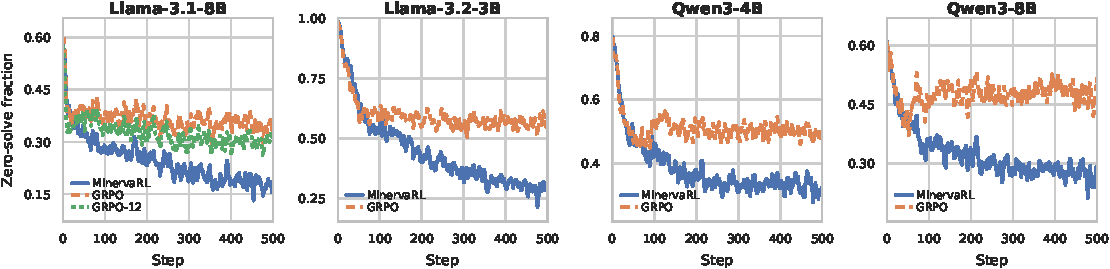
\includegraphics[width=.9\linewidth]{figures/zero_solve_frac_min_1x4.pdf}
  \caption{Fraction of prompts whose rollout group has maximum verifier reward $=0$. Each panel compares GRPO and MinervaRL; Llama-3.1-8B also includes GRPO-12 ($N=12$). Curves use a 5-step rolling mean.}
  \label{fig:zero-solve-fraction}
\end{figure}

\begin{figure}[!t]
  \centering
  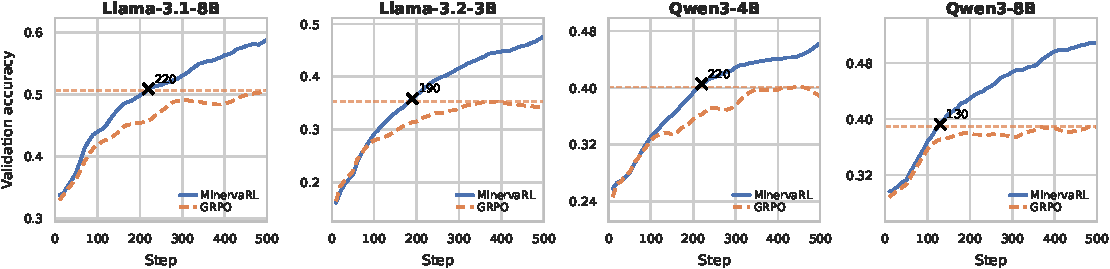
\includegraphics[width=.9\linewidth]{figures/valacc_1x4.pdf}
  \caption{Validation accuracy over training. Curves are 5-step rolling means; dashed lines mark the best GRPO accuracy, and crosses mark the first MinervaRL step that reaches it.}
  \label{fig:validation-accuracy-dynamics}
\end{figure}

\Cref{fig:validation-accuracy-dynamics} shows that the reduction in zero-solve prompts is accompanied by improved validation performance. Across all four backbones, MinervaRL reaches the best GRPO validation accuracy during training and then continues improving beyond it. This indicates that the support-seeding mechanism does more than change rollout diversity: it converts sparse-reward prompts into useful training signal that improves verifier-scored validation accuracy.








\subsection{General Capability and Structured-Output Transfer}
\label{sec:other-benchmarks-transfer}




\begin{table}[!t]
\centering
\scriptsize
\caption{Additional evaluations: Llama-3.1-8B general/cyber benchmarks and Qwen2.5-Coder-3B text-to-SQL transfer. Higher is better except WMDP-Cyber. Underlined values indicate the best score in each column.}
\label{tab:additional-evals}
\begin{minipage}[t]{0.43\linewidth}
\centering
\textbf{(a) Other benchmarks}\par\vspace{2pt}
\setlength{\tabcolsep}{2pt}
\renewcommand{\arraystretch}{0.9}
\resizebox{\linewidth}{!}{%
\begin{tabular}{@{}l c c c c@{}}
\toprule
Model & \shortstack{MMLU\\Pro $\uparrow$} & IFEval $\uparrow$ & \shortstack{Canary\\Exploit $\uparrow$} & \shortstack{WMDP\\Cyber $\downarrow$} \\
\midrule
Llama-3.1-8B & 44.1 & 72.3 & 10.9 & 46.7 \\
Llama-Primus & 41.5 & 68.2 & \underline{29.8} & 46.3 \\
Foundation-Sec & 42.5 & 67.1 & 0.0 & \underline{45.3} \\
Llama-3.1-8B-GRPO & \underline{45.6} & 72.3 & 0.0 & 47.1 \\
Llama-3.1-8B-MinervaRL & 43.6 & \underline{73.8} & 28.4 & 47.1 \\
\bottomrule
\end{tabular}%
}
\end{minipage}
\hfill
\begin{minipage}[t]{0.54\linewidth}
\centering
\textbf{(b) Text-to-SQL transfer}\par\vspace{2pt}
\setlength{\tabcolsep}{2pt}
\renewcommand{\arraystretch}{0.9}
\resizebox{\linewidth}{!}{%
\begin{tabular}{@{}l c c c c c c c c@{}}
\toprule
Model & \shortstack{Spider\\Dev} & \shortstack{Spider\\Test} & \shortstack{BIRD\\Dev} & DK & Syn & Real. & Live & Avg \\
\midrule
Qwen2.5-Coder & 77.4 & 77.6 & 50.3 & 65.6 & 67.2 & \underline{69.7} & 3.7 & 58.8 \\
SQL-R1-3B & 77.1 & 77.4 & 53.3 & \underline{70.5} & 67.5 & 66.5 & 6.3 & 59.8 \\
GRPO & 77.5 & 78.5 & \underline{54.2} & 69.0 & 67.9 & 68.7 & 6.3 & 60.3 \\
MinervaRL & \underline{78.2} & \underline{79.3} & 52.5 & 69.2 & \underline{70.7} & 69.3 & \underline{6.7} & \underline{60.8} \\
\bottomrule
\end{tabular}%
}
\end{minipage}
\end{table}

We include two auxiliary evaluations: general/cyber benchmarks for Llama-3.1-8B variants and a preliminary text-to-SQL transfer experiment. \Cref{tab:additional-evals}(a) shows that MinervaRL largely preserves MMLU-Pro~\citep{wang2024mmlu} and IFEval~\citep{zhou2023instruction} performance, improves CanaryExploit~\citep{bhatt2024cyberseceval} over the base and GRPO variants, and does not increase WMDP-Cyber~\citep{li2024wmdp} relative to GRPO, where lower scores indicate lower measured cyber-risk.

\Cref{tab:additional-evals}(b) evaluates transfer to text-to-SQL, another structured-output setting with executable or verifier-style rewards. Starting from Qwen2.5-Coder-3B, we train GRPO and MinervaRL using the SQL-R1~\citep{ma2025sqlr1} training/validation setup and compare against the base model and SQL-R1-3B. MinervaRL obtains the best average score (60.8) and leads on four of seven datasets, suggesting that MinervaRL can provide gains beyond CTI in structured-output domains with sparse or long-tail verifiable rewards.










\subsection{Ablations and Hyperparameter Sensitivity}
\label{sec:ablations}



\begin{table}[!t]
\centering
\scriptsize
\caption{Ablations and sensitivity analysis. Underlined values indicate the best score in each comparison block.}
\label{tab:ablation-summary}
\setlength{\tabcolsep}{2.2pt}
\renewcommand{\arraystretch}{0.88}
\begin{tabular}{@{}lccc@{\hspace{0.9em}}cccc@{}}
\toprule
\multicolumn{4}{c}{\textbf{(a) Baselines and ablations}}
&
\multicolumn{4}{c}{\textbf{(b) Distillation scale}} \\
\cmidrule(r){1-4}
\cmidrule(l){5-8}
Approach
& \shortstack{Minerva-\\Dev}
& \shortstack{AthenaBench-\\Mini}
& Avg
& $\gamma$
& \shortstack{Minerva-\\Dev}
& \shortstack{AthenaBench-\\Mini}
& Avg \\
\midrule
Base                  & 18.2 & 43.0 & 30.6
& 0.01 & 60.3 & 61.3 & 60.8 \\
GRPO                  & 50.3 & 57.4 & 53.8
& 0.02 & 63.1 & 63.3 & 63.2 \\
GRPO (12 rollouts)    & 50.9 & 52.7 & 51.8
& 0.05 & \underline{63.2} & \underline{63.3} & \underline{63.3} \\
SFT (answer-only)     & 58.6 & 38.7 & 48.7
& 0.10 & 60.1 & 58.1 & 59.1 \\
MinervaRL             & 63.2 & \underline{63.3} & \underline{63.3}
&      &      &      &      \\
\midrule
No EMA teacher        & 63.1 & 62.2 & 62.6
&      &      &      &      \\
No filtering          & 63.0 & 61.4 & 62.2
&      &      &      &      \\
No ML filter          & \underline{64.2} & 59.0 & 61.6
&      &      &      &      \\
\bottomrule
\end{tabular}
\end{table}



\Cref{tab:ablation-summary}(a) tests whether MinervaRL's gains can be matched by simpler alternatives or attributed to a single component. Increasing the GRPO rollout budget from $N=8$ to $N=12$ does not close the gap to MinervaRL, indicating that the improvement is not explained by additional exploration alone. Direct answer-only SFT improves Minerva-Dev but performs much worse on AthenaBench-Mini, suggesting that final-answer imitation is less robust than verifier-guided RL augmented with trace distillation. Component ablations further show that the full MinervaRL pipeline gives the strongest average performance: removing the EMA teacher, removing all filtering, or removing only the ML filter each reduces the average score.

\Cref{tab:ablation-summary}(b) shows sensitivity to the distillation learning-rate scale $\gamma$ used in the supervised update, with learning rate $\gamma\cdot \mathrm{lr}_{\mathrm{rlvr}}$. Performance is best around $\gamma=0.05$: smaller values under-use accepted traces, while a larger value degrades both validation splits. We therefore use $\gamma=0.05$ in the main experiments.














% \begin{figure}[!t]
%   \centering
%   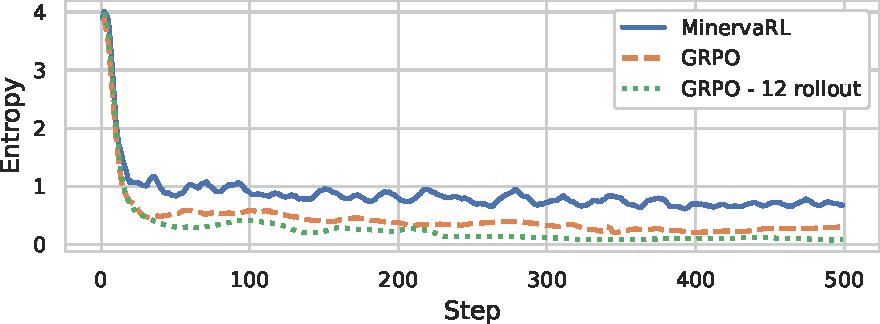
\includegraphics[width=0.8\linewidth]{figures/llama8b-entropy.pdf}
%   \caption{Policy entropy over training for Llama-8B-Instruct.}
%   \label{fig:entropy-over-training}
% \end{figure}



% \paragraph{Entropy.}
% \Cref{fig:entropy-over-training} shows that MinervaRL retains relatively higher policy entropy than GRPO during training.
% This helps maintain exploration and reduces the risk of prematurely collapsing onto narrow response patterns, which is particularly important under sparse verifiable rewards.

